\section{Разработка программно-аппаратного комплекса}

\subsection{Серверная аппаратная часть}
Для выбора серверной аппаратной части нужно опираться, в первую очередь, на системные
требования используемого на кафедре ПО. Для оценки в таблице \ref{tab:solid_req}
приводятся системные требования основного используемого на кафедре КПРС САПР SolidWorks
с сайта разработчика Dassault Systems \cite{ref:solid_req2} \cite{ref:solid_req1}.

\begin{table}[htpb]
    \centering
    \caption{Системные требования Solidworks}
    \label{tab:solid_req}
    \begin{tabularx}{\linewidth}{Xr}
        \toprule
        Процессор & 3.3 ГГц или выше \\
        RAM & 16 ГБ или более \\
            & 32 ГБ рекомендуется для Simulation \\
            & и работы с большими сборками \\
        Устройство хранения & рекомендуется SSD \\
        Место на диске & 20 ГБ и более \\
        \bottomrule
    \end{tabularx}
\end{table}

Требования для многопользовательской работы не указаны, поэтому нужно провести
дополнительные исследования производительности системы при многопользовательской работе.
По предварительным испытаниям компьютер кафедры обеспечивает достаточную
производительность для базовой работы в Soldiworks двух подключенных клиентов.

\subsection{Клиентская аппаратная часть}
Для работы в качестве тонкого клиента подходит практически любой x86-совместимый
компьютер, на котором есть возможность запустить клиент нужного протокола.
Соответственно, существующие на кафедре компьютеры могут быть использованы в качестве
ТК. Однако, для получения многих преимуществ ТК есть смысл использовать более
компактные и энергоэффективные системы.

В качестве основной платформы для разработки ТК будет использован одноплатный компьютер
Raspberry Pi 3B. Его характеристики приведены в таблице \ref{tab:rpi_specs}, внешний вид
— на рисунке \ref{pic:piphoto}.

\begin{table}[h]
    \centering
    \caption{Технические характеристики Raspberry Pi 3B}
    \label{tab:rpi_specs}
    \begin{tabularx}{\linewidth}{Xr}
        \toprule
        Процессор & однокристальный чип Broadcom BCM2837 \\
        микроархитектура & ARM Cortex-A53 \\
        разрядность & 64-бит \\
        количество ядер & 4 \\
        тактовая частота & 1,2 ГГц \\
        оперативная память & 1ГБ LPDDR2 SDRAM \\
        \midrule
        цифровой видеовыход & HDMI \\
        композитный выход & 3,5 мм (4 pin) \\
        USB порты & USB 2.0×4 \\
        сеть & WiFi 802.11n, 10/100 Мб RJ45 Ethernet \\
        Bluetooth & Bluetooth 4.1, Bluetooth Low Energy \\
        разъем дисплея & Display Serial Interface (DSI) \\
        разъем видеокамеры & MIPI Camera Serial Interface (CSI-2) \\
        карта памяти & MicroSD \\
        порты ввода-вывода & 40 \\
        габариты & 85x56x17 мм \\
        \bottomrule
    \end{tabularx}
\end{table}

\begin{figure}[h]
    \center
    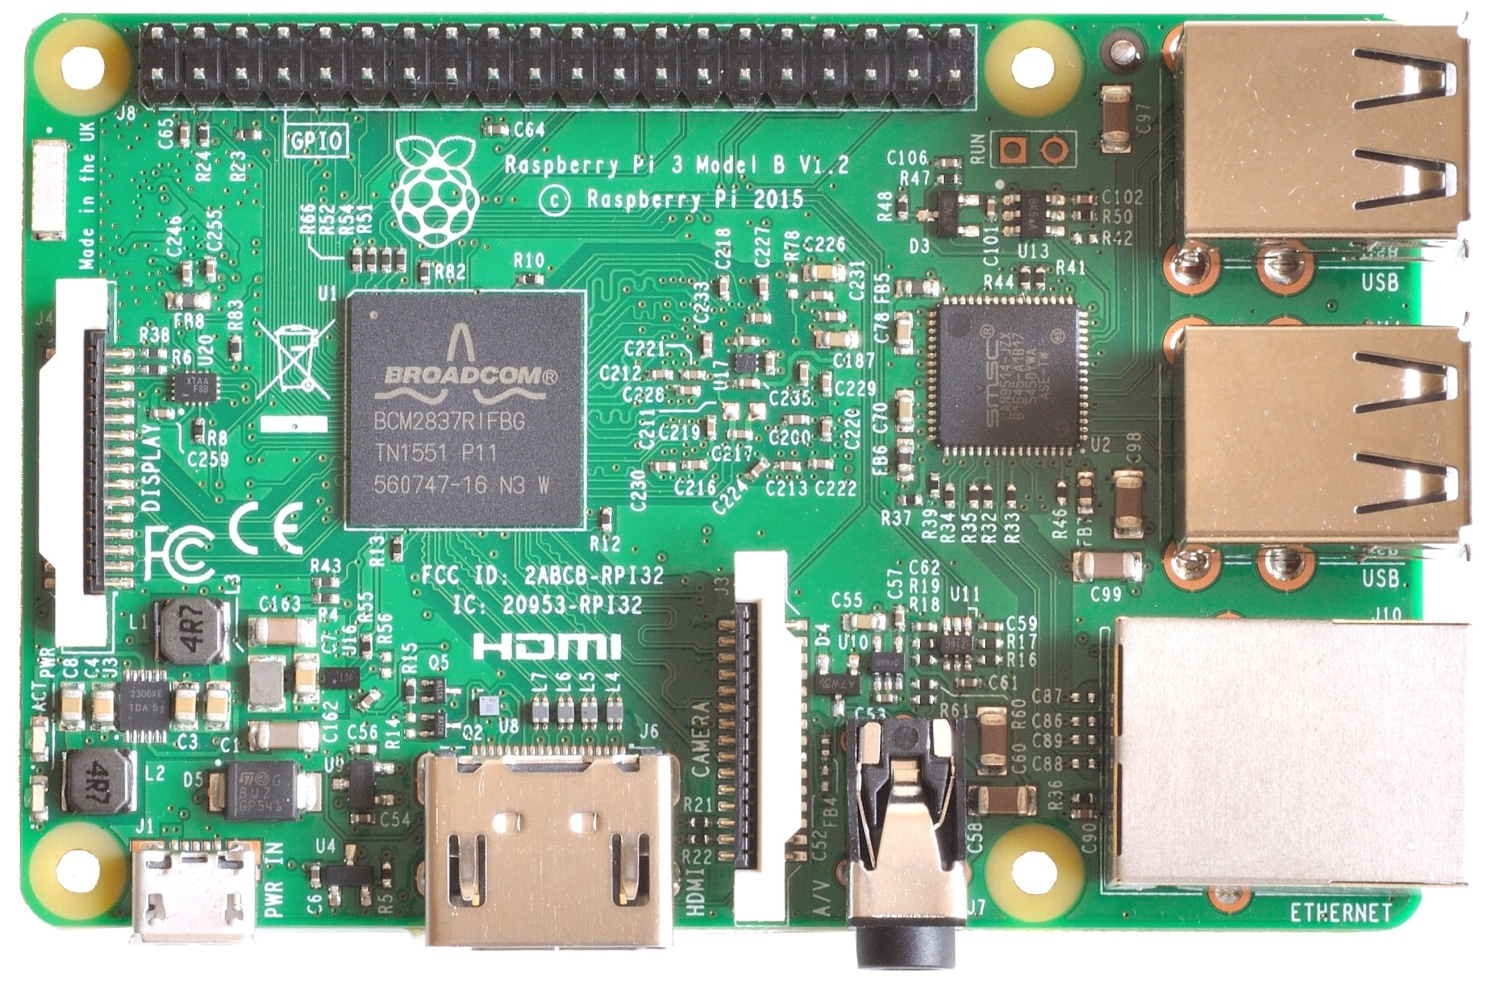
\includegraphics[width=\linewidth]{piphoto}
    \caption{Внешний вид Raspberry Pi 3B}
    \label{pic:piphoto}
\end{figure}

К недостаткам такого решения относятся:
\begin{itemize}
    \item Отсутствие в комплекте поставки корпуса, блока питания, SD-карты.
    \item Невозможность использования аппаратного ускорения графики, т.к. отсутствуют 
        драйвера с открытым исходным кодом для BCM2837.
    \item Производительность зависит от нагрева процессора, необходимость качественного
        охлаждения.
    \item ARM архитектура снижает количество доступного ПО (по сравнению с
        x86-совместимыми устройствами).
\end{itemize}

Стоит отметить, что эти недостатки будут частично устранены при разработке данного
проекта.
По результатам предварительных исследований, производительности Raspberry Pi 3B
достаточно для использования в этом проекте.

\subsection{Выбор используемого протокола}

Для разработки необходимо выбрать способ удаленного доступа, который будет
использоваться в системе. Так как выбор зависит от серверной ОС, выбор оптимального
варианта связан с доступными на Windows протоколами.

Основной протокол, используемый в Windows — RDP (Remote Desktop Protocol). Клиент RDP
доступен во всех редакциях Windows, начиная с Windows XP, что позволяет использовать
любой компьютер кафедры в качестве тонкого клиента (см. рисунок \ref{pic:mstsc_xp}).
Однако, RDP-клиенты существуют для многих платформ, в том числе для Linux.

\begin{figure}[h]
    \center
    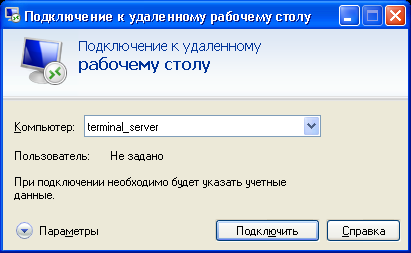
\includegraphics[height=8cm]{mstsc_xp}
    \caption{Окно RDP-клиента, встроенного в Windows XP}
    \label{pic:mstsc_xp}
\end{figure}

\subsection{Клиентское ПО}

В качестве клиентской ОС выбран стандартный для Raspberry Pi дистрибутив Linux Raspbian,
основанный на Debian \cite{ref:raspbian}.
Дистрибутив поддерживается Raspberry Pi Foundation и рекомендован к установке.
К его преимуществам можно отнести открытый исходный код, простоту установки и удобство 
настройки. 
Актуальной на момент разработки была версия Buster, вышедшая в феврале 2020 года.

Для RDP-клиента использовано ПО freerdp, актуальной на момент разработки версии
2.0.0. Данный программный продукт позволяет осуществлять подключение к RDP-серверам
любой версии, просто и гибко настраивается для получения оптимальной производительности.
Так как исходный код открыт, есть возможность скомпилировать бинарный файл для нужной
архитектуры (в рассматриваемом проекте используется архитектура ARM).
